\documentclass[12pt,fleqn]{article}\usepackage{../common}
\begin{document}
Lineer Cebir - Ders 3

Onceki derslerde matris carpimi yaptik, bu derste bu islemin kurallarini
gorecegiz. Bu isi pek cok sekilde yapmanin yolu var ve hepsi onemli, ve
ayni sonucu veriyor.

Sonra matris tersi (inverse) konusuna girecegiz, orada bir suru kavram var,
ve cok onemli. 

Iki matrisi carpma teknigiyle baslayalim. 

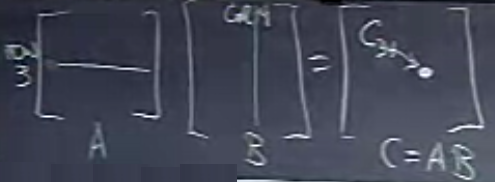
\includegraphics[height=4cm]{3_01.png}

Bu carpimi yaparken soldaki matrisin uzerinde sol isaret parmagi,
sagdakinde sag isaret parmagi konulur, ve soldan-saga, yukaridan-asagi iki
el hareket ettirilir, ve gosterilen hucreler birbiri ile carpilir, bu
carpimlar toplanir. Ustte soldaki matrisin 3. satiri, sagdaki matrisin
4. kolonu baz alinmis, bu carpim ve toplama sonucu $C$'nin 3. satir ve
4. kolonundaki degeri elde ederiz. Bu degere $c_{34}$ diyelim,

$$ 
\left[\begin{array}{rrrr}
\\
\\
a_{31} & a_{32} & \dots \\
\\
\\
\end{array}\right]
\left[\begin{array}{rrrrr}
& & b_{14} & & \\
& & b_{24} & & \\
& &  & & \\
& &  & & \\
& &  & & 
\end{array}\right] 
=
\left[\begin{array}{rrrrr}
& &  & & \\
& &  & & \\
& & c_{34} & & \\
& &  & & \\
& &  & & 
\end{array}\right]
$$

$$ c_{34} = \textrm{ 3. satir } \times \textrm{ 4. kolon } $$

$$ = a_{31}b_{14} + a_{32}b_{24} + ... $$















\end{document}
